At first glance, the simulations appear to be approximately resolution-independent, relaxing to a similar disk relatively quickly.

Of particular interest is the scale height of the disk between the {\tt custom\_lowres}, {\tt custom}, and {\tt custom\_highres} runs.
These are calculated by fitting an exponential profile,
\begin{equation}
    \rho_x(z) \propto \mathrm{sech}^2\left(z/Z_x\right)
    \label{eqn:vertprofile}
\end{equation}
with $Z_x$ the scale height for component $x$. The results are shown in Figure \ref{fig:vheighthist}.

The differences between the two regimes can be understood through a simple \citet{jeans_stability_1902} analysis; the central regions have a considerably higher density and hence smaller Jeans length.
This, according to \citet{schaye_model-independent_2001}, implies that the scale height should be considerably smaller.
It is possible to use the simulations as a test of the aforementioned work, by calculating the local 3D density ($\rho_g$), surface density ($\sg$), and Jeans' length ($L_J$).
These values are presented in Table \ref{tab:schaye_test} and show that whilst the Jeans' length and actual scale height are roughly of order each other in low density regions, in the high density regions this approximation quickly becomes invalid.
This appears to be resolution-independent, however the {\tt custom\_highres} model shows a considerably higher density central region due to the reduced softening length.

Whilst the assertion from \citet{schaye_model-independent_2001} that $\sg \approx \rho_g L_J$ is tested somewhat by these data, the {\tt custom} simulations still produce a more accurate scale height for the disk of $Z_g \approx 100 \pc$ than the $\approx 1$ kpc found in the {\tt default} simulations.
This is possibly explained through the differing phases that each of these models are designed to reproduce.
The {\tt default} model aims to represent all of the gas in the galaxy, from the cold neutral medium through to the hot ionized medium.
The {\tt custom} model, in comparison, aims only to represent the warm medium and below; hence the smaller scale height.

\begin{table}
    \centering
    \resizebox{\textwidth}{!}{
    \begin{tabular}{l|c|c|c|c|c|c}
        Run & Range [kpc] & $\rho_g$ [n$_H$ cm$^{-3}$] & $\sg$ [$\mathrm{M}_\odot \pc^{-2}$] & $\sg/\rho_g$ [pc] & $L_J$ [pc] & $Z_g$ [pc] \\
        \hline

        {\tt custom} & $r<0.5$ & 7.06$\times10^3$ & 3.4$\times10^3$ & 19.5 & 34.7 &  26.3 \\
        {\tt custom\_highres} & $r<0.5$ & 5.79$\times10^5$ & 3.51$\times10^3$ & 0.245 & 3.85 &  7.89 \\
        {\tt custom\_lowres} & $r<0.5$ & 5.31$\times10^3$ & 3.34$\times10^3$ & 25.4 & 39.8 &  29.9 \\
        {\tt default} & $r<0.5$ & 12 & 93.7 & 315 & 410 &  345 \\
        {\tt default\_lowres} & $r<0.5$ & 5.76 & 47.4 & 333 & 517 &  261 \\
        {\tt custom} & $0.5<r<5$ & 79.3 & 10 & 5.1 & 102 &  69.8 \\
        {\tt custom\_highres} & $0.5<r<5$ & 111 & 6.12 & 2.23 & 78.1 &  54.2 \\
        {\tt custom\_lowres} & $0.5<r<5$ & 132 & 8.32 & 2.55 & 76.2 &  82.5 \\
        {\tt default} & $0.5<r<5$ & 1.38 & 15.8 & 464 & 848 &  756 \\
        {\tt default\_lowres} & $0.5<r<5$ & 0.732 & 15.4 & 849 & 1.16$\times10^3$ &  436 \\


\end{tabular}}
\caption{Values comparing possible measures of scale height for the different runs, with $r$ corresponding to galactocentric radius. The local densities ($\rho_g$) are calculated by taking the mean density computed by GADGET-2 over all of the contained particles.}
    \label{tab:schaye_test}
\end{table}


\begin{figure}
    \centering
    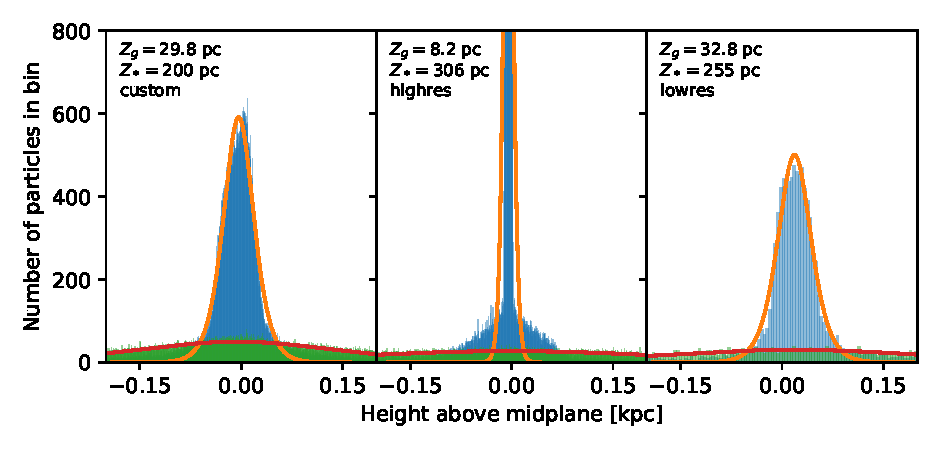
\includegraphics{v_height_hist.pdf}
    \caption{The vertical distribution of the particles in the disk (for {\tt custom}, {\tt custom\_highres} and {\tt custom\_lowres}) after $\approx 2$ Gyr of evolution from the initial conditions. The top set of histograms encompasses all of the data, whereas the bottom set exclude the particles residing within the inner $0.5$ kpc of the galaxy. In blue and orange, the gas histogram and fit are shown, with the same for the star particles being shown in green and red. The fits use the density profile in Equation \ref{eqn:vertprofile}, with $Z_g$ the scale height of the gas and $Z_*$ the scale height of the stellar disk. The {\tt custom\_lowres} is shown with bins ten times as wide as to normalise the overall contents of the histogram. It appears that the scale height of the gas disk is determined by the chosen softening length, as the {\tt custom\_highres} run has a considerable build up of particles within the very centre of the disk. Normally, the disk is spread vertically by the ejection from supernovae explosions, and as these are not modelled in a local way in the {\tt custom} model a high degree of clumping is shown. From the splitting of the histograms, it is clear that there are two regimes here; the inner $\approx 0.5$ kpc, and the rest of the galaxy. The inner region (see Figure \ref{fig:sd_r_evo}) contains the majority of the mass in the galaxy, and as such the gaseous disk is highly compressed (the {\tt custom\_highres} run shows this in most detail because of the smaller gravitational softening). This suggests that the model presented in this work does not account for all of the dynamics in the galaxy, which is to be expected due to its inherent simple nature.}
    \label{fig:vheighthist}
\end{figure}
